% IEEE standard conference template; to be used with:
%   spconf.sty  - LaTeX style file, and
%   IEEEbib.bst - IEEE bibliography style file.
% --------------------------------------------------------------------------
\documentclass[letterpaper]{article}
\usepackage{spconf,amsmath,amssymb,graphicx,listings,hyperref,array,float,epstopdf,tikz}
\lstset{basicstyle=\ttfamily\footnotesize,numbers=left,stepnumber=2,frame=single,language=c,captionpos=b}
\usepackage[utf8]{inputenc} % UTF-8 was invented to be used.
\usetikzlibrary{positioning}
\usetikzlibrary{shadows}


% Example definitions.
% --------------------
% nice symbols for real and complex numbers
\newcommand{\R}[0]{\mathbb{R}}
\newcommand{\C}[0]{\mathbb{C}}

% make document compile with \todo comments
\newcommand{\todo}{\\}

% bold paragraph titles
\newcommand{\mypar}[1]{{\bf #1.}}

% Title.
% ------
\title{Parallel XML Query Processing using XML Stream Compression}
%
% Single address.
% ---------------
\name{Serge Balzan, Stefan Dietiker, Tobias Kaiser}
\address{Department of Computer Science\\ ETH Z\"urich\\Z\"urich, Switzerland}

% For example:
% ------------
%\address{School\\
%		 Department\\
%		 Address}
%
% Two addresses (uncomment and modify for two-address case).
% ----------------------------------------------------------
%\twoauthors
%  {A. Author-one, B. Author-two\sthanks{Thanks to XYZ agency for funding.}}
%		 {School A-B\\
%		 Department A-B\\
%		 Address A-B}todo
%  {C. Author-three, D. Author-four\sthanks{The fourth author performed the work
%		 while at ...}}
%		 {School C-D\\
%		 Department C-D\\
%		 Address C-D}
%

\begin{document}
%\ninept
%
\maketitle
%

The hard page limit is 6 pages in this style. Do not reduce font size
or use other tricks to squeeze. This pdf is formatted in the American letter format, so the spacing may look a bit strange when printed out.

\begin{abstract}
Describe in concise words what you do, why you do it (not necessarily
in this order), and the main result.  The abstract has to be
self-contained and readable for a person in the general area. You
should write the abstract last.
\end{abstract}




\section{Introduction}\label{sec:intro}

In this report we describe the results of our project that was part of the
course ''Design of Parallel and High Performance Computing'' at ETH Z\"urich.
The goal of the project was to develop a parallel implementation of an important
algorithm or application, that scales well in a multicore environment. This
report describes an approach to process large XML files or data streams in
parallel using the XPath query language.

XML is most commonly used as an interoperable file exchange format and as such
is used in a wide variety of fields, from documents formats, such as Open
Document Format \todo{ref} and or XHTML \todo{ref} to various kinds of
configuration file formats. All of these applications have in common that XML is
primarily used as a general tool to persist and restore the dynamic state of an
application program.

Following the on-going trend towards big data, however, XML has also been used
to make large amounts of structured data available as high throughput streams.
One such example is Twitter Firehose which makes all user generated tweets
available trough a single XML-Stream\footnote{Twitter has changed the document
format from XML to JSON. We point out that the techniques presented in this
report can easily be adapted to work with almost any structured data exchange
format.}. Twitter Firehose reaches a throughput of up to 3 Gbps.

Most off-the-shelf are single-threaded and tailored towards the applications
mentioned above. Processing structured data at such a high throughput, however,
only becomes possible by leveraging the power of multi processor systems. As
parsing is an inherently sequential process, this requires the careful
orchestration of parallel processors.

Ideally, the data can be split into chunks than can be processed independently.
In our approach we achieve this by using a compression that is agnostic of the
internal structure of the XML data. The XPath query matching is done using the
compressed data.

Our implementation focuses on XML query matching, using XPath. It is written in
C/C++ and our platform of choice is the Intel's Xeon Phi, incorporating 61 cores
and 16 GB of memory. We found a scalable approach to process queries on large
XML files. Our implementation reaches a throughput of about 0.93 GB/s and offers
a big potential for optimization to the architecture at use. 

\mypar{Related work} Main inspiration of our work was \cite{Ogden2013}. Ogden et
al describe an approach to query XML data with the help of pushdown transducers.
Its core idea is to generate mappings of a start state and an end state. For
each chunk one mapping is being computed and then, when each core has finished
processing its part, they are merged according to the matching end and start
states of each chunk.

Optimally to process XML streams, deterministic automatons are used. The
compilation of XPath queries into automatons is discussed in \cite{Green2004}.


%\mypar{Motivation} Nowadays, in the age of the internet of things and social
%media, where a lot and continuous information is being generated and every
%single person has the opportunity to share their thoughts and insights, a huge
%content of valuable information is available. One of these examples is the
%Twitter Firehose, which generates an output of all tweet being made in real
%time. The data stream may reach an output rate of 3 Gbps and more on  its peak,
%therefore to process this data in real time requires high computational power.
%
%To achieve the necessary processing power, one can use a multicore chip, that
%provides several processing units, that work in parallel. While dealing with
%such a datastream or data file in sequential is trivial and straight-forward, an
%implementation in parallel is not as simple. The data formats used are mostly
%context-free languages, such as XML or JSON. To operate on the stream in
%parallel, it must be splitted into similar chunks and distributed to each core.
%Ideally, these chunks are well-formed and self-contained, such that no
%processing unit requires to exchange any information with other units. To
%generate well-formed chunks, parsing and preprocessing the data beforehand
%sequentially is necessary. As this might pose a bottleneck for parallel and
%high-performance query matching on XML data, in our approach we try to avoid any
%preprocessing on the raw data. Thus we had to find a way, in which each unit is
%able to operate on its chunk without any additional information from its peers.


\section{Background: Whatever the Background is}\label{sec:background}

Give a short, self-contained summary of necessary
background information. For example, assume you present an
implementation of sorting algorithms. You could organize into sorting
definition, algorithms considered, and asymptotic runtime statements. The goal of the
background section is to make the paper self-contained for an audience
as large as possible. As in every section
you start with a very brief overview of the section. Here it could be as follows: In this section 
we formally define the sorting problem we consider and introduce the algorithms we use
including a cost analysis.

\mypar{Sorting}
Precisely define sorting problem you consider.

\mypar{Sorting algorithms}
Explain the algorithm you use including their costs.

As an aside, don't talk about "the complexity of the algorithm.'' It's incorrect,
problems have a complexity, not algorithms.


\section{Your Proposed Method}\label{sec:yourmethod}

Now comes the ``beef'' of the report, where you explain what you
did. Again, organize it in paragraphs with titles. As in every section
you start with a very brief overview of the section.

In this section, structure is very important so one can follow the technical content.

Mention and cite any external resources that you used including libraries or other code.


\section{Experimental Results}\label{sec:exp}

Here we present the results of our experiment conducted to measure the performance of the main parts of the system, the tokenizer and the matcher. First a description of the setup to run the benchmarks followed by a short explanation of the experiments and finally the results.

\mypar{Experimental Setup} The experiments were executed on an Intel Xeon Phi 7120 coprocessor. It consists of 61 cores and 16 GB of GDDR5 memory with a theoretical bandwidth of 352 GB/s. According to the documentation the Xeon Phi's optimal computational power can be reached running two threads per core, i.e. 120 threads.
For compilation the Intel Compiler version 15.0.0 20140723 was used with the following flags: \verb;-fopenmp; \verb;-std=c++11; \verb;-mmic; \verb;-Wall; \verb;-qopt-report3; \\ \verb;-qopt-report-phase=vec; \verb;-O3;.

The benchmarks focus on the tokenizer and the matcher. To generate test data, we used the XML benchmark project XMark \cite{Schmidt2002}. To measure the scalability of the tokenizer 100 test runs were conducted. For each run, an input file of the size of 2 GB was used which contained 61'113'640 tokens. First, we measured the performance of the tokenizer working with 1 thread. Then we increased the number of threads to 2, 4, 8, 16, 32, 60, 120, 180 and 240. Each experiment was run ten times. The results were built with the average of these runs. Similarly, the matcher was tested with files of the sizes 2 GB (27'620'104 tokens), 4 GB (55'236'244 tokens) and 8 GB (110'467'124 tokens). For each file 10 different experiments were run. The first experiment matched 1 query, i.e. running with 1 thread, the second matched 2 queries and the following experiments matched 4, 8, 16, 32, 60, 120, 180 and 240 queries. Again, the result is the average of the runs.

\mypar{Results}
The experiments reveal clearly, that the throughput of the tokenizer increases with the number of threads. In figure ~\ref{tokenizer_throughput}, where the throughput against the number of threads is plotted, nearly linear scaling can be observed. While the benefits of more threads are significant up to 120 threads, i.e. two threads per core, less performance can be gained from 120 up to 240 threads. These results confirm the optimal use of processors, which is at two threads per core, as we mentioned earlier.

\begin{figure}[h]\centering
  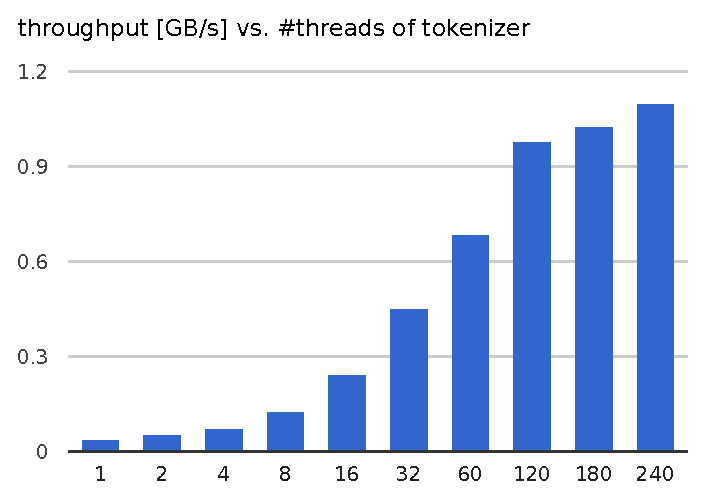
\includegraphics[scale=.66]{img/tokenizer_throughput_2.eps}
  \caption{Throughput of the tokenizer in GB/s measured with different numbers of threads.
  \label{tokenizer_throughput}}
\end{figure}

In figure~\ref{matcher_throughput} the throughput of the matcher against the numbers of queries, i.e. threads, is plotted. Since the file size alone does not reveal enough information about the complexity, or the number of tokens in the XML data, the throughput is given in the number of tokens that are processed per second. Until up to 60 queries there is no significant drop of the performance, while with 120 queries and more the throughput plummets. Weak scaling is observable for up to 60 threads. When the number of threads exceeds the number of cores the performance suffers. The sudden decrease of performance for 8 GB might be due to the memory access pattern on the Xeon Phi, which becomes apparent, when more threads operate at the same time on larger amount of data. Pursuing experiments that confirm this hypothesis would exceed the format of this report. 

\begin{figure}[h]\centering
  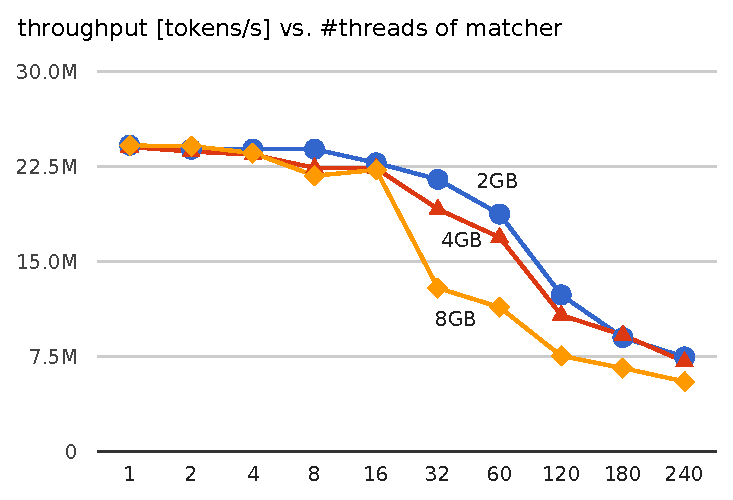
\includegraphics[scale=.66]{img/matcher_throughput_2.eps}
  \caption{Throughput of the matcher in tokens/s comparing different input sizes. \label{matcher_throughput}}
\end{figure}

A direct comparison of the processing time of the tokenizer and the matcher is plotted in figure ~\ref{matcher_tokenizer_pt}. The numbers represent the absolute processing time of a XML file of 2 GB. One can see, that the processing time of the matcher stays practically the same, even when increasing the numbers of queries being processed, while decreasing drastically for the tokenizer when more threads are provided.

\begin{figure}[h]\centering
  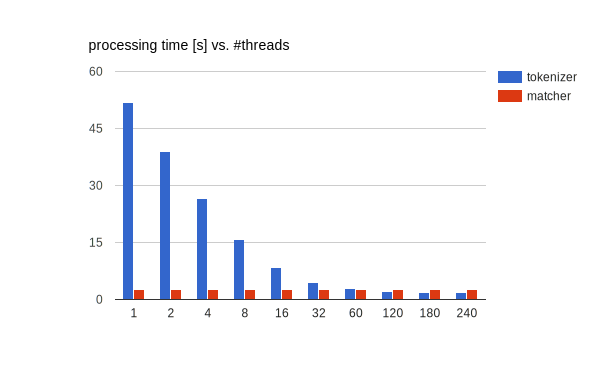
\includegraphics[scale=.66]{img/matcher_tokenizer_p_time.eps}
  \caption{Processing time of matcher and tokenizer in comparison for an input of size 2 GB.
  \label{matcher_tokenizer_pt}}
\end{figure}

The total throughput of the tokenizer and matcher running with 120 threads is 0.29 GB/s.
\todo{Exact Data / Experiment basis for 0.29GB/s value?}
\section{Conclusions}

We implemented a parallel and high performance XPath query matcher using compression to minimize data usage. Our goal was to reach strong scaling within the tokenizer and weak scaling of the matcher. As mentioned before, both of these goals were reached. Even though only a subset of XPath was considered, the experiments are still meaningful, as our system can be extended to, such that the full XPath query language can be processed with similar results. Also our approach is not limited to XML, but can also be used for different context free languages, such as JSON, in combination with a similar query language, like JSONPath.

When comparing our results to other, similar, approaches, such as \cite{Ogden2013}, one must consider, that the priorities were set differently. While Ogden et al focus on data parallelism and trade it for the complexity and number of queries, our implementation emphasizes query parallelism. Also a direct comparison with the same data is not meaningful, as the used architecture differ entirely.

To enhance performance, different techniques for the compression could be used, which might result in a higher throughput of the system. Also the system has still a high potential on being optimized for the underlying hardware.
\input{06_appendix.tex}

\section{Further comments}

Here we provide some further tips.

\mypar{Further general guidelines}

\begin{itemize}
\item For short papers, to save space, I use paragraph titles instead of
subsections, as shown in the introduction.

\item It is generally a good idea to break sections into such smaller
units for readability and since it helps you to (visually) structure the story.

\item The above section titles should be adapted to more precisely
reflect what you do.

\item Each section should be started with a very
short summary of what the reader can expect in this section. Nothing
more awkward as when the story starts and one does not know what the
direction is or the goal.

\item Make sure you define every acronym you use, no matter how
convinced you are the reader knows it.

\item Always spell-check before you submit (to us in this case).

\item Be picky. When writing a paper you should always strive for very
high quality. Many people may read it and the quality makes a big difference.
In this class, the quality is part of the grade.

\item Books helping you to write better: \cite{Higham:98} and \cite{Strunk:00}.

\item Conversion to pdf (latex users only): 

dvips -o conference.ps -t letter -Ppdf -G0 conference.dvi

and then

ps2pdf conference.ps
\end{itemize}

\mypar{Graphics} For plots that are not images {\em never} generate the bitmap formats
jpeg, gif, bmp, tif. Use eps, which means encapsulate postscript. It is
scalable since it is a vector graphic description of your graph. E.g.,
from Matlab, you can export to eps.

The format pdf is also fine for plots (you need pdflatex then), but only if the plot was never before in the format 
jpeg, gif, bmp, tif.


% References should be produced using the bibtex program from suitable
% BiBTeX files (here: bibl_conf). The IEEEbib.bst bibliography
% style file from IEEE produces unsorted bibliography list.
% -------------------------------------------------------------------------
\bibliographystyle{IEEEbib}
\bibliography{bibl_conf}

\end{document}

